\chapter{Projekt: Středisko Keya 2021} % (fold)
\label{cha:projekt_středisko_keya_2021}

Pro někoho to možná bude úplnou novinkou, pro jiného potvrzením spekulací, a někdo to třeba už dávno věděl, každopádně přišel čas na to vyslat tuto informaci oficiálně do světa – na přelomu roku 2020 a 2021 se oddíly Anpetu a Hanyetu oddělí od Blaníku a dají vzniknout samostatnému středisku Keya.

Je to informace, která může znít poměrně převratně, nicméně faktem je, že pro většinu zúčastněných o nějaký velký převrat nejde. Členové oddílů ani jejich rodiče pravděpodobně nepoznají rozdíl, alespoň půjde-li vše tak, jak doufáme. Největší změna to tak bude pro samotné vedoucí v oddílech, pro které se změní ledasco, ovšem snad jenom k lepšímu.

Jak jsme k rozhodnutí o této na první pohled možná kosmetické změně dospěli? Naším primárním důvodem je skutečnost, že Blaník se svými stovkami členů se nám čím dál více stával finančním a technickým správcem a přestával být skautskou rodinnou. Ono udržovat vztahy s patnácti dalšími oddíly rozesetými po celé Praze zkrátka a dobře není v lidských silách. Po loňském rozdělení Keyi na dva oddíly se pro nás navíc stalo mnohem důležitějším udržet úzké vazby hlavně mezi sebou. A když se k tomu přidá skutečnost, že máme vlastní klubovnu a objevila se skupina zkušených vedoucích, kteří jsou ochotní se budoucímu středisku Keya věnovat, nic nebrání tomu, abychom se do zakládání pustili.

Jak to bude celé probíhat? V uplynulém roce probíhaly diskuse o tom, jakým způsobem bychom chtěli, aby naše středisko fungovalo. Tyto diskuse se stanou základním kamenem práce vznikajícího střediskového vedení. Zároveň jsme se domluvili s vedením Blaníku na jízdním řádu „Kexitu“ – během jara zkompletujeme tým vedení střediska, od příštího skautského roku (to je od podzimu 2020) začneme fungovat nezávisle na Blaníku, a s novým rokem kalendářním dojde i k oddělení právnímu a finančnímu.

\begin{center}
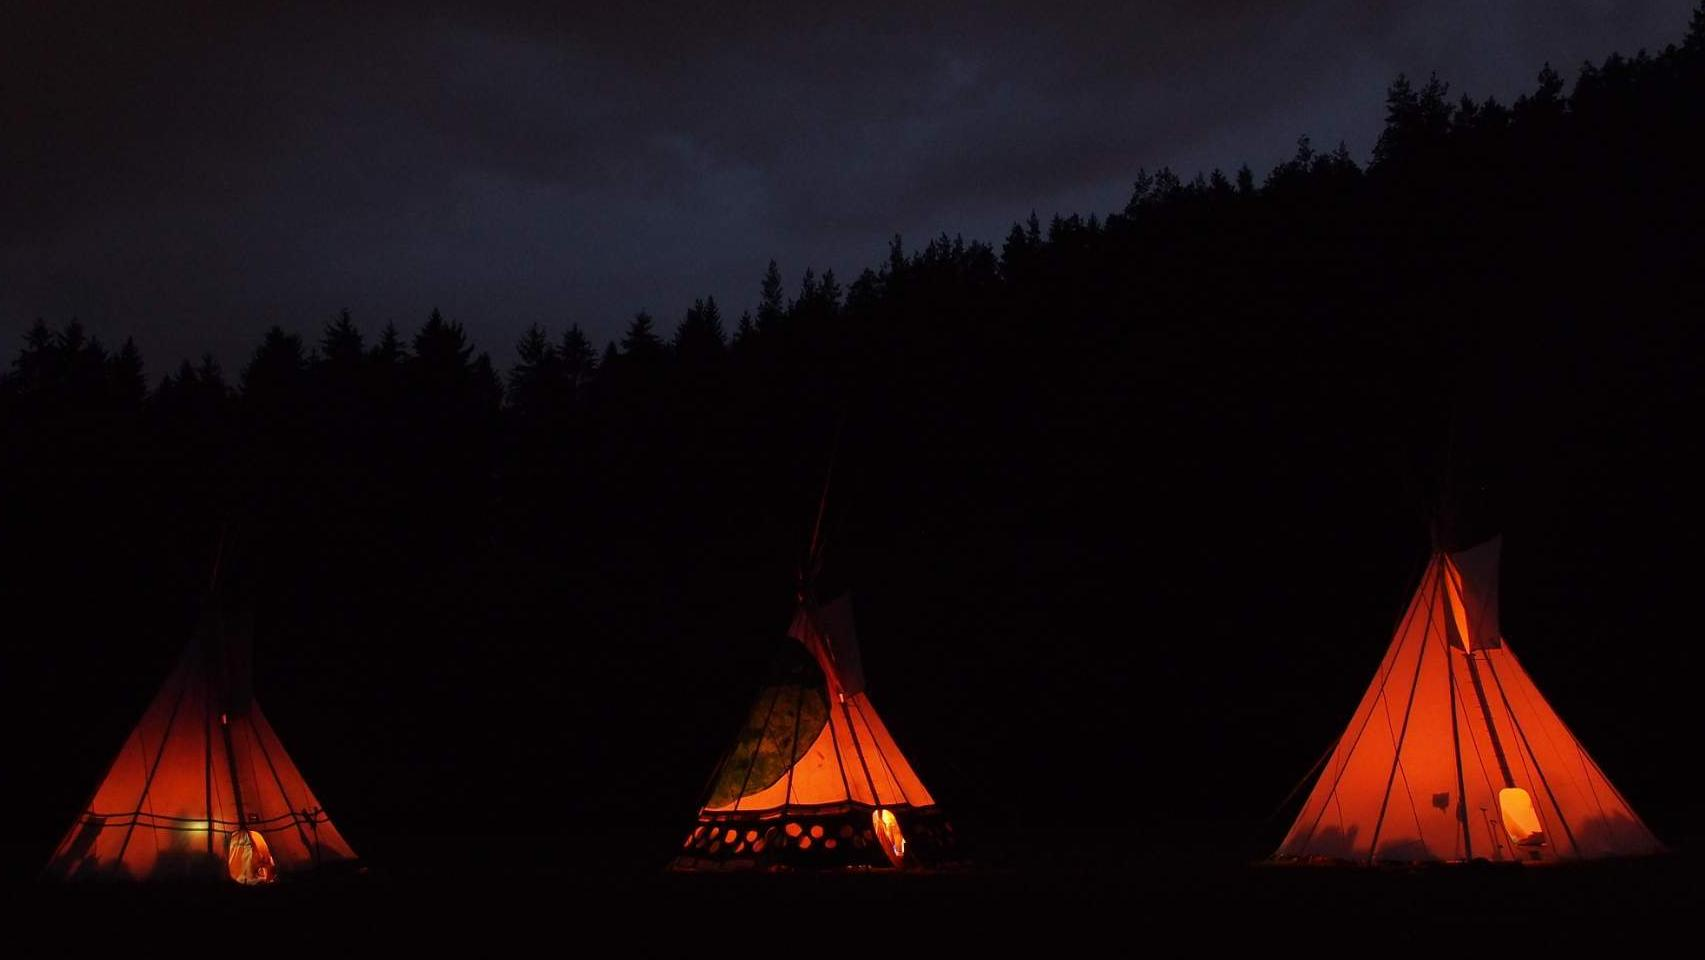
\includegraphics[width=9cm]{img/udo_clanky/fikuv_clanek_stredisko.jpg}
\end{center}

Dobrou zprávou je, že se celý projekt nese v pozitivním duchu. Naše oddělení není vynucené a ani k němu nedochází z důvodu, že bychom měli nějaké spory s Blaníkem. Věříme sice, že v užším kruhu se nám bude lépe dařit udržovat vzájemné vztahy a budeme snad i fungovat o něco efektivněji, ale rozhodně neodcházíme ve zlém či s pocitem povýšenosti. Spíše na to všechno hledíme jako na výzvu, která nám jistě přinese mnohé problémy a komplikace, ale na kterou se s chutí vrhneme. Tak nám držte palce, budeme to potřebovat!

\podpis{Fík}

\clearpage

% chapter projekt_středisko_keya_2021 (end)